%==============================================================================
% Tento soubor použijte jako základ
% This file should be used as a base for the thesis
% Autoři / Authors: 2008 Michal Bidlo, 2022 Jaroslav Dytrych
% Kontakt pro dotazy a připomínky: sablona@fit.vutbr.cz
% Contact for questions and comments: sablona@fit.vutbr.cz
%==============================================================================
% kódování: UTF-8 (zmena prikazem iconv, recode nebo cstocs)
% encoding: UTF-8 (you can change it by command iconv, recode or cstocs)
%------------------------------------------------------------------------------
% zpracování / processing: make, make pdf, make clean
%==============================================================================
% Soubory, které je nutné upravit nebo smazat: / Files which have to be edited or deleted:
%   projekt-20-literatura-bibliography.bib - literatura / bibliography
%   projekt-01-kapitoly-chapters.tex - obsah práce / the thesis content
%   projekt-01-kapitoly-chapters-en.tex - obsah práce v angličtině / the thesis content in English
%   projekt-30-prilohy-appendices.tex - přílohy / appendices
%   projekt-30-prilohy-appendices-en.tex - přílohy v angličtině / appendices in English
%==============================================================================
\documentclass[]{fitthesis} % bez zadání - pro začátek práce, aby nebyl problém s překladem
%\documentclass[english]{fitthesis} % without assignment - for the work start to avoid compilation problem
%\documentclass[zadani]{fitthesis} % odevzdani do IS VUT a/nebo tisk s barevnými odkazy - odkazy jsou barevné
%\documentclass[english,zadani]{fitthesis} % for submission to the IS VUT and/or print with color links - links are color
%\documentclass[zadani,print]{fitthesis} % pro černobílý tisk - odkazy jsou černé
%\documentclass[english,zadani,print]{fitthesis} % for the black and white print - links are black
%\documentclass[zadani,cprint]{fitthesis} % pro barevný tisk - odkazy jsou černé, znak VUT barevný
%\documentclass[english,zadani,cprint]{fitthesis} % for the print - links are black, logo is color
% * Je-li práce psaná v anglickém jazyce, je zapotřebí u třídy použít 
%   parametr english následovně:
%   If thesis is written in English, it is necessary to use 
%   parameter english as follows:
%      \documentclass[english]{fitthesis}
% * Je-li práce psaná ve slovenském jazyce, je zapotřebí u třídy použít 
%   parametr slovak následovně:
%   If the work is written in the Slovak language, it is necessary 
%   to use parameter slovak as follows:
%      \documentclass[slovak]{fitthesis}
% * Je-li práce psaná v anglickém jazyce se slovenským abstraktem apod., 
%   je zapotřebí u třídy použít parametry english a enslovak následovně:
%   If the work is written in English with the Slovak abstract, etc., 
%   it is necessary to use parameters english and enslovak as follows:
%      \documentclass[english,enslovak]{fitthesis}

% Základní balíčky jsou dole v souboru šablony fitthesis.cls
% Basic packages are at the bottom of template file fitthesis.cls
% zde můžeme vložit vlastní balíčky / you can place own packages here
\usepackage{afterpage}

\newcommand\blankpage{%
    \null
    \thispagestyle{empty}%
    \addtocounter{page}{-1}%
    \newpage}

% Pro seznam zkratek lze využít balíček Glossaries - nutno odkomentovat i níže a při kompilaci z konzoly i v Makefile (plnou verzi pro Perl, nebo lite)
% The Glossaries package can be used for the list of abbreviations - it is necessary to uncomment also below. When compiling from the console also in the Makefile (full version for Perl or lite)
%\usepackage{glossaries}
%\usepackage{glossary-superragged}
%\makeglossaries 

% Nastavení cesty k obrázkům
% Setting of a path to the pictures
%\graphicspath{{obrazky-figures/}{./obrazky-figures/}}
%\graphicspath{{obrazky-figures/}{../obrazky-figures/}}

%---rm---------------
\renewcommand{\rmdefault}{lmr}%zavede Latin Modern Roman jako rm / set Latin Modern Roman as rm
%---sf---------------
\renewcommand{\sfdefault}{qhv}%zavede TeX Gyre Heros jako sf
%---tt------------
\renewcommand{\ttdefault}{lmtt}% zavede Latin Modern tt jako tt

% vypne funkci šablony, která automaticky nahrazuje uvozovky,
% aby nebyly prováděny nevhodné náhrady v popisech API apod.
% disables function of the template which replaces quotation marks
% to avoid unnecessary replacements in the API descriptions etc.
\csdoublequotesoff

\usepackage{url}

% =======================================================================
% balíček "hyperref" vytváří klikací odkazy v pdf, pokud tedy použijeme pdflatex
% problém je, že balíček hyperref musí být uveden jako poslední, takže nemůže
% být v šabloně
% "hyperref" package create clickable links in pdf if you are using pdflatex.
% Problem is that this package have to be introduced as the last one so it 
% can not be placed in the template file.
\ifWis
\ifx\pdfoutput\undefined % nejedeme pod pdflatexem / we are not using pdflatex
\else
  \usepackage{color}
  \usepackage[unicode,colorlinks,hyperindex,plainpages=false,pdftex]{hyperref}
  \definecolor{hrcolor-ref}{RGB}{223,52,30}
  \definecolor{hrcolor-cite}{HTML}{2F8F00}
  \definecolor{hrcolor-urls}{HTML}{092EAB}
  \hypersetup{
	linkcolor=hrcolor-ref,
	citecolor=hrcolor-cite,
	filecolor=magenta,
	urlcolor=hrcolor-urls
  }
  \def\pdfBorderAttrs{/Border [0 0 0] }  % bez okrajů kolem odkazů / without margins around links
  \pdfcompresslevel=9
\fi
\else % pro tisk budou odkazy, na které se dá klikat, černé / for the print clickable links will be black
\ifx\pdfoutput\undefined % nejedeme pod pdflatexem / we are not using pdflatex
\else
  \usepackage{color}
  \usepackage[unicode,colorlinks,hyperindex,plainpages=false,pdftex,urlcolor=black,linkcolor=black,citecolor=black]{hyperref}
  \definecolor{links}{rgb}{0,0,0}
  \definecolor{anchors}{rgb}{0,0,0}
  \def\AnchorColor{anchors}
  \def\LinkColor{links}
  \def\pdfBorderAttrs{/Border [0 0 0] } % bez okrajů kolem odkazů / without margins around links
  \pdfcompresslevel=9
\fi
\fi
% Řešení problému, kdy klikací odkazy na obrázky vedou za obrázek
% This solves the problems with links which leads after the picture
\usepackage[all]{hypcap}


% Informace o práci/projektu / Information about the thesis
%---------------------------------------------------------------------------
\projectinfo{
  %Prace / Thesis
  project={BP},            %typ práce BP/SP/DP/DR  / thesis type (SP = term project)
  year={2023},             % rok odevzdání / year of submission
  date=\today,             % datum odevzdání / submission date
  %Nazev prace / thesis title
  title.cs={Detekce komunikace malware v síťových \\tocích},  % název práce v češtině či slovenštině (dle zadání) / thesis title in czech language (according to assignment)
  title.en={Detection of Malware Communication in Network Flows}, % název práce v angličtině / thesis title in english
  %title.length={14.5cm}, % nastavení délky bloku s titulkem pro úpravu zalomení řádku (lze definovat zde nebo níže) / setting the length of a block with a thesis title for adjusting a line break (can be defined here or below)
  %sectitle.length={14.5cm}, % nastavení délky bloku s druhým titulkem pro úpravu zalomení řádku (lze definovat zde nebo níže) / setting the length of a block with a second thesis title for adjusting a line break (can be defined here or below)
  %dectitle.length={14.5cm}, % nastavení délky bloku s titulkem nad prohlášením pro úpravu zalomení řádku (lze definovat zde nebo níže) / setting the length of a block with a thesis title above declaration for adjusting a line break (can be defined here or below)
  %Autor / Author
  author.name={Václav},   % jméno autora / author name
  author.surname={Korvas},   % příjmení autora / author surname 
  %author.title.p={Bc.}, % titul před jménem (nepovinné) / title before the name (optional)
  %author.title.a={Ph.D.}, % titul za jménem (nepovinné) / title after the name (optional)
  %Ustav / Department
  department={UIFS}, % doplňte příslušnou zkratku dle ústavu na zadání: UPSY/UIFS/UITS/UPGM / fill in appropriate abbreviation of the department according to assignment: UPSY/UIFS/UITS/UPGM
  % Školitel / supervisor
  supervisor.name={Ondřej},   % jméno školitele / supervisor name 
  supervisor.surname={Ryšavý},   % příjmení školitele / supervisor surname
  supervisor.title.p={doc. Ing.},   %titul před jménem (nepovinné) / title before the name (optional)
  supervisor.title.a={Ph.D.},    %titul za jménem (nepovinné) / title after the name (optional)
  % Klíčová slova / keywords
  keywords.cs={Sem budou zapsána jednotlivá klíčová slova v českém (slovenském) jazyce, oddělená čárkami.}, % klíčová slova v českém či slovenském jazyce / keywords in czech or slovak language
  keywords.en={Sem budou zapsána jednotlivá klíčová slova v anglickém jazyce, oddělená čárkami.}, % klíčová slova v anglickém jazyce / keywords in english
  %keywords.en={Here, individual keywords separated by commas will be written in English.},
  % Abstrakt / Abstract
  abstract.cs={Do tohoto odstavce bude zapsán výtah (abstrakt) práce v českém (slovenském) jazyce.}, % abstrakt v českém či slovenském jazyce / abstract in czech or slovak language
  abstract.en={Do tohoto odstavce bude zapsán výtah (abstrakt) práce v anglickém jazyce.}, % abstrakt v anglickém jazyce / abstract in english
  %abstract.en={An abstract of the work in English will be written in this paragraph.},
  % Prohlášení (u anglicky psané práce anglicky, u slovensky psané práce slovensky; u projektové praxe lze zakomentovat) / Declaration (for thesis in english should be in english; for project practice can be commented out)
  declaration={Prohlašuji, že jsem tuto bakalářskou práci vypracoval samostatně pod vedením pana X...
Další informace mi poskytli...
Uvedl jsem všechny literární prameny, publikace a další zdroje, ze kterých jsem čerpal.},
  %declaration={I hereby declare that this Bachelor's thesis was prepared as an original work by the author under the supervision of Mr. X
% The supplementary information was provided by Mr. Y
% I have listed all the literary sources, publications and other sources, which were used during the preparation of this thesis.},
  % Poděkování (nepovinné, nejlépe v jazyce práce; nechcete-li, zakomentujte pro skrytí nadpisu) / Acknowledgement (optional, ideally in the language of the thesis; comment out for hiding including heading)
  acknowledgment={V této sekci je možno uvést poděkování vedoucímu práce a těm, kteří poskytli odbornou pomoc
(externí zadavatel, konzultant apod.).},
  %acknowledgment={Here it is possible to express thanks to the supervisor and to the people which provided professional help
%(external submitter, consultant, etc.).},
  % Rozšířený abstrakt (cca 3 normostrany) - lze definovat zde nebo níže / Extended abstract (approximately 3 standard pages) - can be defined here or below
  %extendedabstract={Do tohoto odstavce bude zapsán rozšířený výtah (abstrakt) práce v českém (slovenském) jazyce.},
  %extabstract.odd={true}, % Začít rozšířený abstrakt na liché stránce? / Should extended abstract start on the odd page?
  %faculty={FIT}, % FIT/FEKT/FSI/FA/FCH/FP/FAST/FAVU/USI/DEF
  faculty.cs={Fakulta informačních technologií}, % Fakulta v češtině - pro využití této položky výše zvolte fakultu DEF / Faculty in Czech - for use of this entry select DEF above
  faculty.en={Faculty of Information Technology}, % Fakulta v angličtině - pro využití této položky výše zvolte fakultu DEF / Faculty in English - for use of this entry select DEF above
  department.cs={Ústav matematiky}, % Ústav v češtině - pro využití této položky výše zvolte ústav DEF nebo jej zakomentujte / Department in Czech - for use of this entry select DEF above or comment it out
  department.en={Institute of Mathematics} % Ústav v angličtině - pro využití této položky výše zvolte ústav DEF nebo jej zakomentujte / Department in English - for use of this entry select DEF above or comment it out
}

% Rozšířený abstrakt (cca 3 normostrany) - lze definovat zde nebo výše / Extended abstract (approximately 3 standard pages) - can be defined here or above
%\extendedabstract{Do tohoto odstavce bude zapsán výtah (abstrakt) práce v českém (slovenském) jazyce.}
% Začít rozšířený abstrakt na liché stránce? / Should extended abstract start on the odd page?
%\extabstractodd{true}

% nastavení délky bloku s titulkem pro úpravu zalomení řádku - lze definovat zde nebo výše / setting the length of a block with a thesis title for adjusting a line break - can be defined here or above
%\titlelength{14.5cm}
% nastavení délky bloku s druhým titulkem pro úpravu zalomení řádku - lze definovat zde nebo výše / setting the length of a block with a second thesis title for adjusting a line break - can be defined here or above
%\sectitlelength{14.5cm}
% nastavení délky bloku s titulkem nad prohlášením pro úpravu zalomení řádku - lze definovat zde nebo výše / setting the length of a block with a thesis title above declaration for adjusting a line break - can be defined here or above
%\dectitlelength{14.5cm}

% řeší první/poslední řádek odstavce na předchozí/následující stránce
% solves first/last row of the paragraph on the previous/next page
\clubpenalty=10000
\widowpenalty=10000

% checklist
\newlist{checklist}{itemize}{1}
\setlist[checklist]{label=$\square$}

% Kompilace po částech (rychlejší, ale v náhledu nemusí být vše aktuální)
% Compilation piecewise (faster, but not all parts in preview will be up-to-date)
% Další informace viz / For more information see https://www.overleaf.com/learn/latex/Multi-file_LaTeX_projects
% \usepackage{subfiles}

% Nechcete-li, aby se u oboustranného tisku roztahovaly mezery pro zaplnění stránky, odkomentujte následující řádek / If you do not want enlarged spacing for filling of the pages in case of duplex printing, uncomment the following line
% \raggedbottom

\begin{document}
  % Vysazeni titulnich stran / Typesetting of the title pages
  % ----------------------------------------------
  \maketitle
  % Obsah
  % ----------------------------------------------
  \setlength{\parskip}{0pt}
  {\afterpage{\blankpage}}
  {\hypersetup{hidelinks}\tableofcontents}

  
  % Seznam obrazku a tabulek (pokud prace obsahuje velke mnozstvi obrazku, tak se to hodi)
  % List of figures and list of tables (if the thesis contains a lot of pictures, it is good)
  \ifczech
    \renewcommand\listfigurename{Seznam obrázků}
  \fi
  \ifslovak
    \renewcommand\listfigurename{Zoznam obrázkov}
  \fi
    {\hypersetup{hidelinks}\listoffigures}
  \ifczech
    \renewcommand\listtablename{Seznam tabulek}
  \fi
  \ifslovak
    \renewcommand\listtablename{Zoznam tabuliek}
  \fi
  % {\hypersetup{hidelinks}\listoftables}

  % Seznam zkratek / List of abbreviations
  %\ifczech
  %  \renewcommand*\glossaryname{Seznam zkratek}%
  %  \renewcommand*\entryname{Zkratka}
  %  \renewcommand*\descriptionname{Význam}
  %\fi
  %\ifslovak
  %  \renewcommand*\glossaryname{Zoznam skratiek}%
  %  \renewcommand*\entryname{Skratka}
  %  \renewcommand*\descriptionname{Význam}
  %\fi
  %\ifenglish
  %  \renewcommand*\glossaryname{List of abbreviations}%
  %  \renewcommand*\entryname{Abbreviation}
  %  \renewcommand*\descriptionname{Meaning}
  %\fi
  % Definice zkratek - z textu se odkazují např. \Gls{TF–IDF}
  % Definition of abbreviations - referred from the text e.g. \Gls{TF–IDF}
  %\newglossaryentry{TF–IDF}
  %{
  %  name={TF–IDF},
  %  description={Term Frequency-Inverse Document Frequency}
  %}
  % 
  %\setglossarystyle{superragged}
  %\printglossaries


  \ifODSAZ
    \setlength{\parskip}{0.5\bigskipamount}
  \else
    \setlength{\parskip}{0pt}
  \fi

  % vynechani stranky v oboustrannem rezimu
  % Skip the page in the two-sided mode
  \iftwoside
    \cleardoublepage
  \fi

  % Text prace / Thesis text
  % ----------------------------------------------
  \ifenglish
    \input{projekt-01-kapitoly-chapters-en}
  \else
    % Tento soubor nahraďte vlastním souborem s obsahem práce.
%=========================================================================
% Autoři: Michal Bidlo, Bohuslav Křena, Jaroslav Dytrych, Petr Veigend a Adam Herout 2019

% Pro kompilaci po částech (viz projekt.tex), nutno odkomentovat a upravit
%\documentclass[../projekt.tex]{subfiles}
%\begin{document}

\chapter{Úvod}

Se stále rostoucí závislostí dnešní společnosti na internetu a počítačích se z těchto technologií stala neodmyslitelná součást našich životů. 
Ovšem stále častěji jsou tyto technologie zneužívány útočníky, kteří přicházejí stále s novými metodami, jak napadnou počítače uživatelů a narušit tak jejich soukromý a nebo odcizit citlivé informace.
Proto je nutné, aby prostředky pro boj s těmito útoky byly neustále modernizovány a byly co nejúčinější.

Proto programy pro detekci škodlivého softwaru (z anglického malicious software, dále pak už jen zkráceně malware) založené na strojovém učení, které jsou v současné době využívány, vyžadují vhodnou datovou sadu na které se bude model učit a ověřovat svoji validitu.
Cílem této práce tedy je vytvoření vhodného nástroje na tvorbu datových sad, které jsou nezbytné pro tyto metody. %detekce založené na strojovém učení.
A dále je pak porovnání těchto metod a jejich úspěšnosti při detekci škodlivého softwaru.

Hlavním důvodem, proč se zabývat rozpoznáváním jednotlivých druhů malwaru a jejich klasifikací, je jeho nezbytnost a důležitost.
Jelikož je velice nereálné, že by v následujícíh letech vymizela potřeba se před těmito útoky branít. Ba naopak lze předpokládat, že 
bude příbývat stále více nových druhů škodlivého softwaru, a proto je nutné na tyto změny rychle a efektivně reagovat, aby byla zajištěna
bezpečnost uživatelů internetových sítí.

Tato bakalářská práce se skláda ze 4 kapitol. Toho úvodu, který slouží jako nahlédnutí do problematiky, následují dvě samostatné kapitoly a závěru. V kapitola \ref{2.chap} se nejprve seznámíte s dělení škodlivého softwaru do rodin. Následně
je představeno několik současných řešení detekce škodlivého softwaru, které jsou založeny na strojovém učení a jejich údajná přesnost.
V kapitole s číslem \ref{3.chap} je pak přiblížen způsob jakým byly vytvořeny vhodné datové sady a popis vytvořeného nástroje sloužícího k tomuto účelu. V závěru jsou pak zhodnoceny dosavadní výsledky a postup další práce.

\chapter{Malware a způsoby jeho detekce} \label{2.chap}
%Prejmenovat tuto kapitolu
Cca 5 stranky co to vůbec malware je a jak se deli a jaké způsoby na detekci se v současné době používají.
Příklady rodin a nějaké statistiky. Co je statická a dynamická analýza

\section{Malware}
\newpage
\section{Zpusoby detekce zalozene na strojovem uceni}
\newpage
\newpage
\section{Analyza malware static x dynamic}
\newpage

\chapter{Automatické vytváření datových sad} \label{3.chap}
%Proč jsou datasety důležité, popsat můj nástroj na tvorbu datasetů. Co je jeho výstupem a jak funguje. Popsat co jsou pcapy, co se vyskytuje v reportech, co je to sandbox prostredi. proc zrovna tento sandbox, zminit i jine.
%Jedna se o jednudochou pipeline a je na obrazku, jednotlive vstupy a vystupy casti jsou popsany v nasledujicich podkapitolach.

Podstatnou a velice důležitou částí této práce je výběr a tvorba vhodných datových sad (z anglického \textit{datasets}).
Protože v této práci je využito stojového učení, je na vytvoření žádoucí datové sady kladen velký důraz. 
S daty totiž souvisí důveryhodnost dosažených výsledků.
Proto byl pro tvorbu žádoucích datových sad vytvořen nástroj, který bude v následující kapitole představen. 

Tato kapitola tedy pojednává o postupu vytváření datových sad. Nejprve je tento proces zjednodušeně popsán.
Poté jsou zde detailně popsány jednotlivé části tohoto procesu popsány a co je jejich vstupem a výstupem.
A nakonec jsou představeny technologie a programovací jazyk, který byl pro toto vytváření zvolen. 

%Tato kapitola tedy pojednává o vybraném programovacím jazyce a knihovnách používaných pro danou úlohu. 
%Poté je popsána obecný proces vytváření těchto datových sad. A nakonec jsou zde popsány jednotlivé části tohoto procesu a 
%jak vypadá skutečný výstup programu.

\section{Postup vytváření datových sad}
Zjednodušený proces tvorby datasetů lze vidět na obrázku \ref{pipeline}, kde je znázorněno jednoduché schéma procesu, jak vytvořený nástroj pracuje. 

Nejprve tedy nástroj stáhne odpovídající počet malware vzorků z volně dostupného databázového serveru. Tyto vzorky jsou pak poslány na server, kde je provedena dynamická analýza.
Pro každý vzorek se provedou dvě analýzy každá na jiném referenčním stroji.
Po dokončení analýzy vzorků jsou ke každému vzorku staženy dva soubory se zachycenou síťovou kumunikací malwaru v podobě \textit{pcap} souborů a ješte zpráva shrnující analýzu daného vzorku.
Každá část tohoto procesu bude detailně popsáno v následujících sekcích, kde budou uvedy i příklady výstupů a výstupů dílčích částí.\\

\begin{figure}[h]
	\centering
        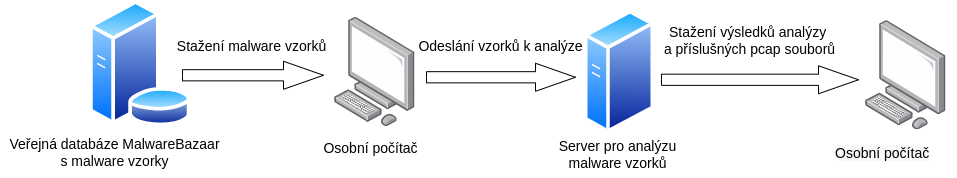
\includegraphics[width=0.8\textwidth]{obrazky/pipeline.png}
	\caption{Proces vytváření datasetů}
    \label{pipeline}
\end{figure}

\section{Stahování malware vzorků}
Prvním krokem je stažení dostatečného počtu malware vzorků pro jednotlivé malware rodiny. Jediným vstupem do toho nástroje od uživatele je tedy pouze textový soubor, který obsahuje
jména rodin. Všechny vzorky jsou stahovány z veřejně dostupné databaze \textit{MalwareBazaar}\footnote{\href{https://bazaar.abuse.ch/}{https://bazaar.abuse.ch/}}. Tato databáze je 
bezplatná a lze stahovat neomezený počet vzorků na rozdíl od jiných databazí jako například \textit{VirusTotal}\footnote{\href{https://www.virustotal.com/gui/home/upload}{https://www.virustotal.com/}}.

Názvy rodin malware musí být stejné jako je specifikuje \textit{MalwareBazaar}, aby nedošlo k nějaké záměně s jiným druhem malwaru. Každý vzorek je poté stažen, jako zaheslovaný zip soubor, aby omylem nedošlo k 
jeho něchtěnému spuštění. Vzorky jsou uloženy podle rodin, aby z důvodu jednoduššího vyhledávání. Jediným omezením je maximalní počet malware vzorků stažených pro jednu rodinu, který činí 1000 vzorků.

\section{Analýza vzorků}
%popsat pcapy, jak probíha analyza, sandboxy
V dalším kroku je nutné veškeré stažené vzorky analyzovat. Každá analýza je prováděna v sandbox prostředení, aby nedošlo k žádnému poškození uživatelského počítače.
Použitým sandbox prostředím pro analýzu je nástroj zvaný \textit{Triage}\footnote{\href{https://tria.ge/dashboard}{https://tria.ge/dashboard}}. Tento nástroj byl vybrán kvůli jeho škálovatelnosti a rychlosti, 
ale především kvůli jeho komplexnímu API rozhraní.

Pro každý vzorek jsou provedeny dvě automatické dynamické analýzy (odkaz na kapitolu) ve dvou různých virtuálních prostředích a jedna statická analýza (ta ovšem není pro tuhle práci tak důležítá, proto se jí dále nebudeme zabývat). 

Celkový proces od nahrání vzorku až po vytoření výsledné zprávy lze vidět na obrázku \ref{Analysis_diagram}. Z něj je patrné, že probíhájí dvě oddělené analýzy. První analýza je prováděno na virtuálním stroji, kde beží 
systém Windows 7 a druhá analýza je prováděna v prostředí se systémem Windows 10.

\begin{figure}[h]
	\centering
        \includegraphics[width=0.6\textwidth]{obrazky/diagram.pdf}
	\caption{Proces analýzy malware vzorků}
    \label{Analysis_diagram}
\end{figure}

Poté, co je vzorek odeslán k analýze, tak je nejprve naplánovaná jeho statická analýza. Po skončení této analýzy je vzorek odeslán k dynamické analýze. Každá analýza se sestáva z extrakce malware vzorku, ze zip archivu. A jeho následného spuštění v čistém prostředí. Poté je zaznamenávána veškerá síťová komunikace a také veškerá aktivita, ke které dojde.
Z obou analýz je pak vygenerována výsledná zpráva.
\section{Výstup programu}
% Popsat pcapy co je v report souborech a k cemu jsou pcapy asi
% konecny vystup programu, rolozeni struktury
%Jak je možné vidět na obrázku \ref{Analysis_diagram}, tak výstupem, který lze ze sandboxu dostat jsou souhrné výsledky analýzy. Tyto výsledky představují soubor (zpráva, anglicky \textit{report}), který popisuje chování malwaru, 
Jak je možné vidět na obrázku \ref{Analysis_diagram}, tak výstupem po skončení dynamické analýzy jsou různé soubory (nebo-li zprávy, anglicky \textit{reports}). Pro účel téhle práce jsou však důležité pouze dva druhy těchto souborů.

Prvním souborem, který je pro tuhle práci relevantní, je soubor obsahující výstup dynamické analýzy. Triage sandbox poskytuje výsledek této analýzy v několika různých formátech jako je třeba XML, JSON či PDF (výstup reportu, který je pak převeden do formátu PDF lze vidět na obrázku ...).
Formát PDF není vhodný z důvodů dalšího zpracování, které bude v následujících fázích potřebné. Nelze z něj jednodušše programově vytáhnout informace. Proto je výsledek analýzy stažen ve formátu JSON.

Mezi významné informace, které lze z toho souboru vyčíst, patří název malware rodiny a krátky popis této rodiny malware. Dále potom ndikátory kompromitace (\texttt{Indicators of Compromise}, zkráceně IoC), 
jsou to tedy hlavně IP adresy a domény, na které se malware snažil připojit a vést jejich prostřednictvím útok. Dále poté může obsahovat navštívené webové stránky a mnoho dalších informací.

\begin{figure}[h]
	\centering
        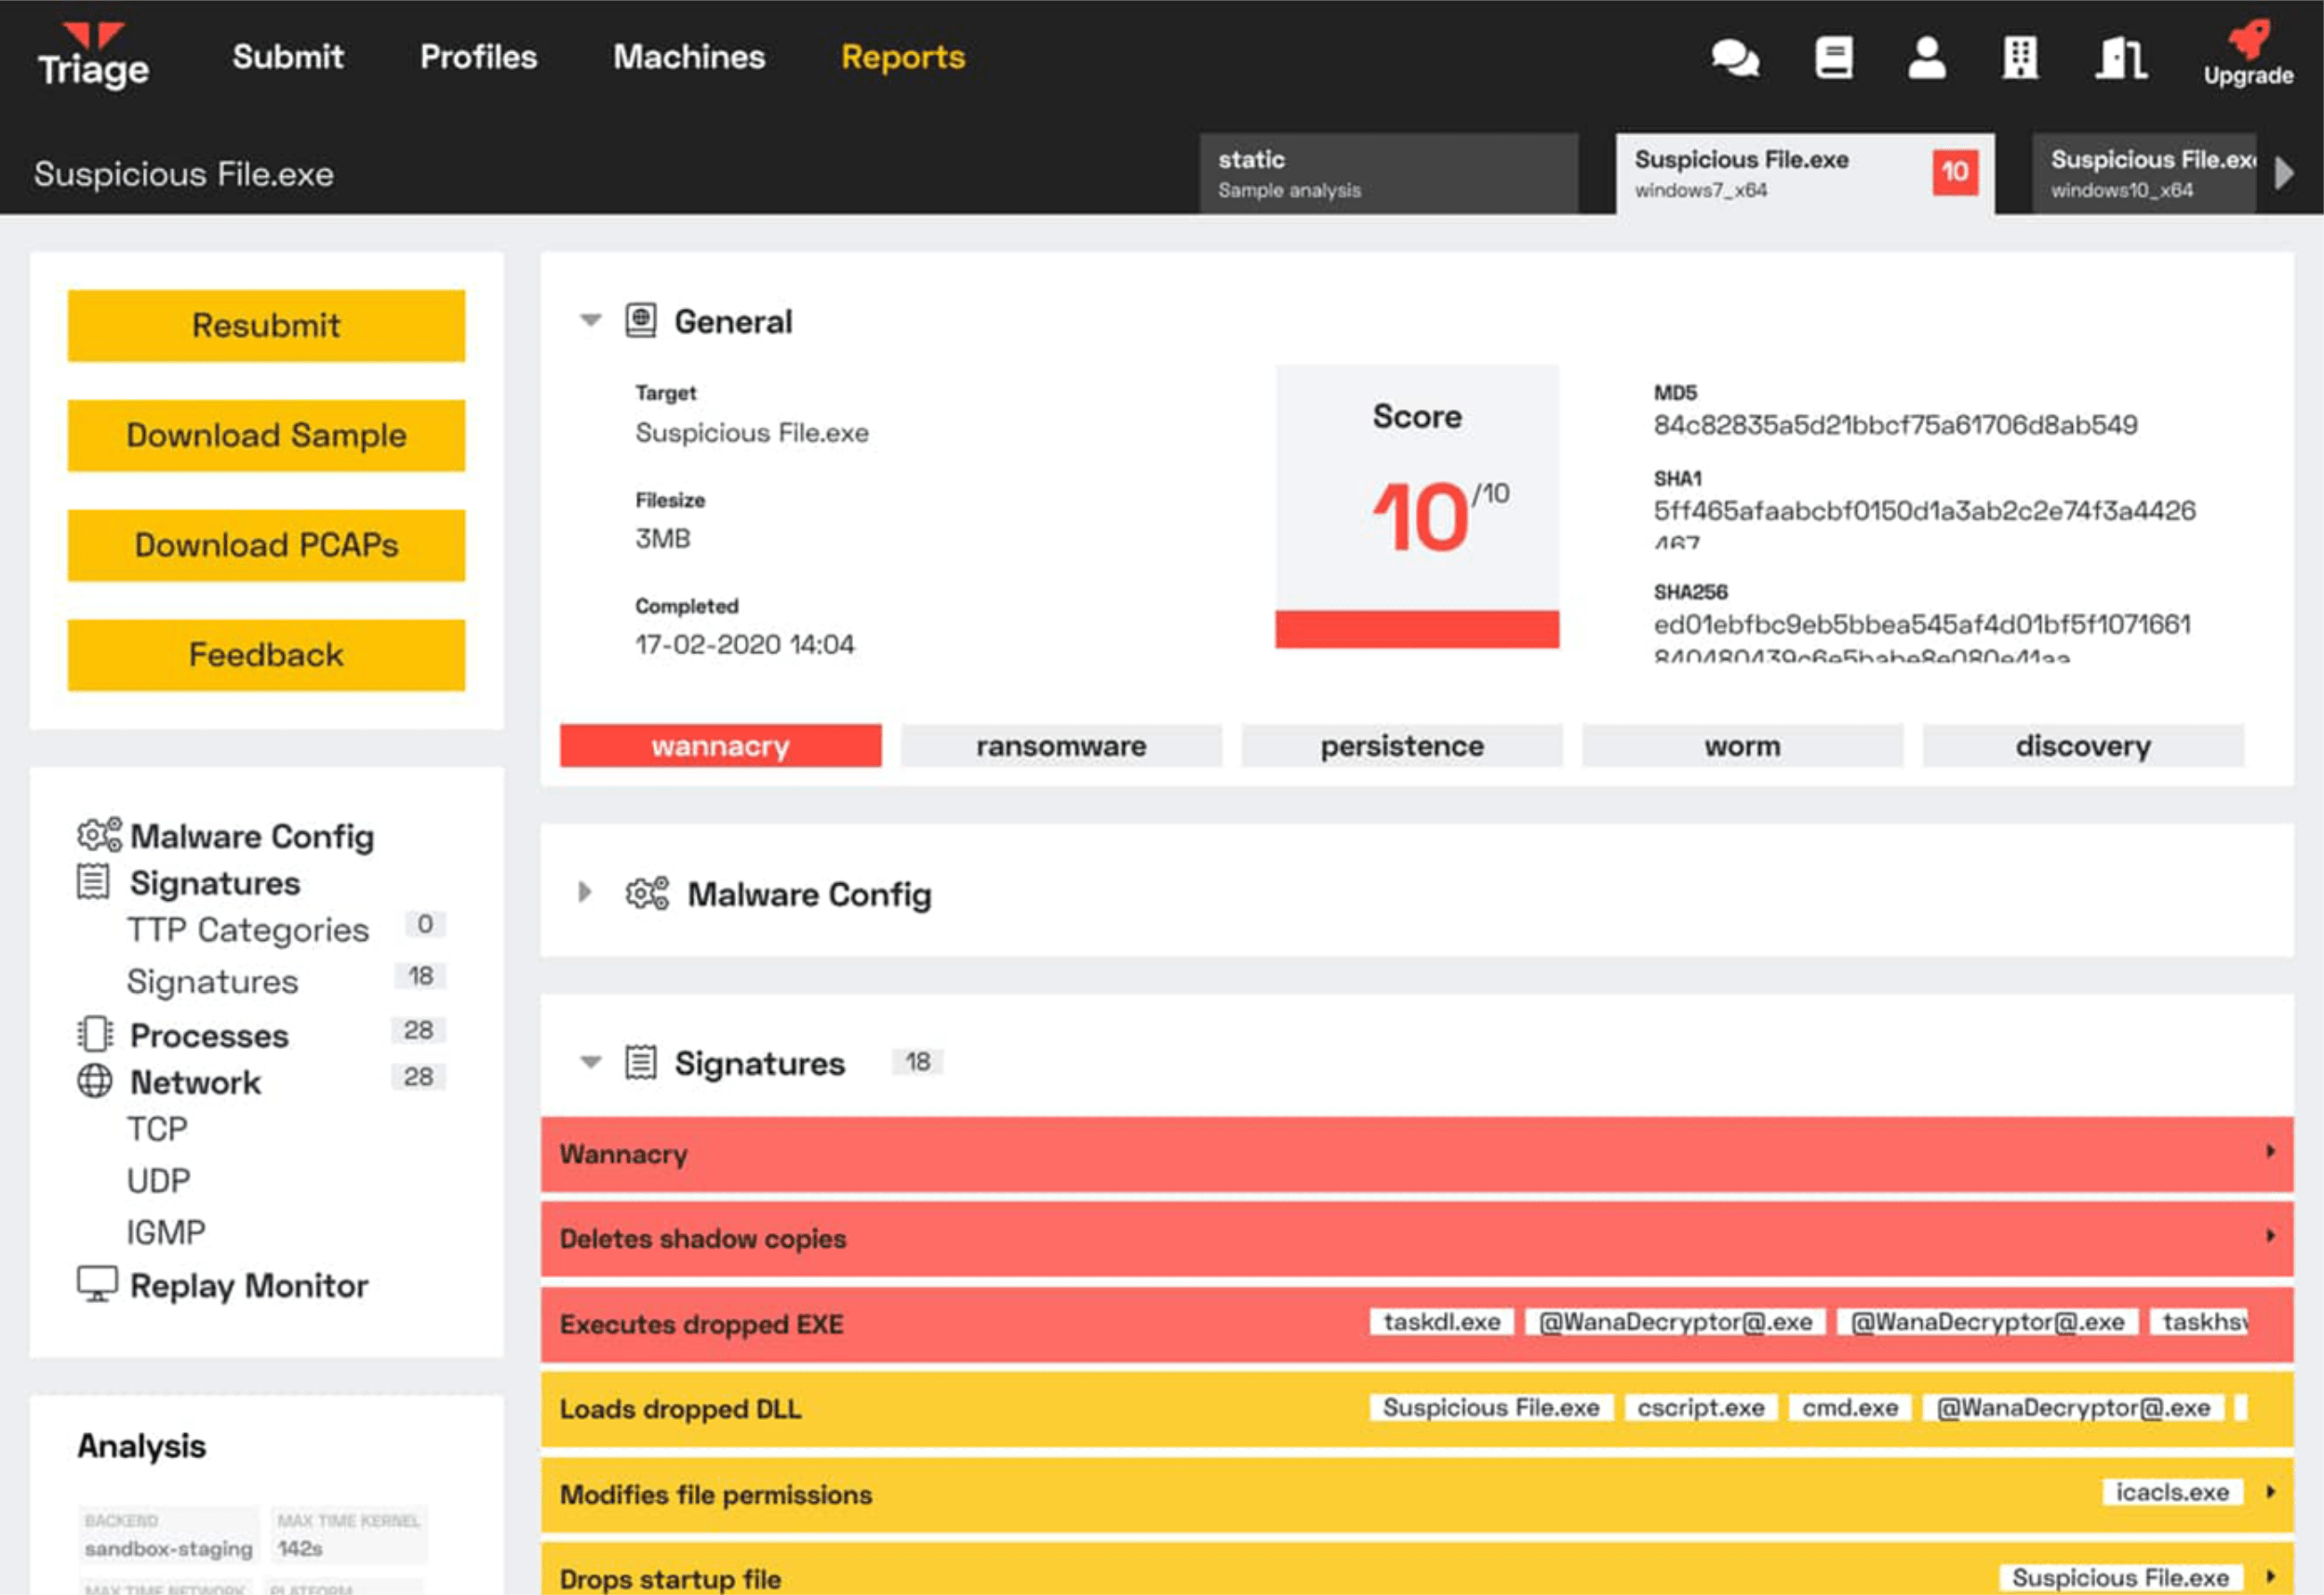
\includegraphics[width=0.7\textwidth]{obrazky/3-triage-report.png}
	\caption{Snímek obrazovky s výsledky z dynamické analýzy}
    \label{Report_image}
\end{figure}

Druhým typem souboru, který je zásadním pro další zpracování jsou soubory typu \texttt{PCAP}. Pro každý malware vzorek jsou staženy dva PCAP soubory.
Tyto soubory obsahují zachycenou síťovou komunikaci ve formě paketů. Tyto soubory lze analyzovat pomocí nástroje \textit{Wireshark}\footnote{\href{https://www.wireshark.org/}{https://www.wireshark.org/}}, 
kde si lze vyfiltrovat komunikaci dle potřeby.

\newpage
\section{Využité technologie}

Veškeré skripty jsou napsány v programovacím jazyce \textbf{Python}. Tento jazyk byl zvolen hned z několika důvodů.
Především ale kvůli jeho jednoduchosti a známosti. Dále taky kvůli knihovnám pro práci s HTTP a posíláním dat po síti.
Velkou výhodou byla také implemetace oficiálního API (aplikačního webového rozhraní z anglického \textit{Application Programming Interface}) klienta pro webové rozhraní 
\texttt{tria.ge}\footnote{\href{https://tria.ge/dashboard}{https://tria.ge/dashboard}}. 
Hlavní využívanou knihovnou je tedy knihovna \textbf{tiage}. Dále se hojně využívá knihovna \textbf{requests} \footnote{\href{https://requests.readthedocs.io/en/latest/}{https://requests.readthedocs.io/en/latest/}}
pro posílaní HTTP požadavků a zpracování jejich odpovědí.

\subsection*{Triage}
Triage je knihovna sloužící ke komunikaci s aplikačním webovým rozhraním Hatching Triage. Tato knihovna usnadňuje práci s analýzou malware vzorků.
Její hlavní použití je tedy odesílaní vzorků k analýze a následné stáhnutí statických výsledků této analýzy a souborů se zachycenou síťovou komunikací v 
podobě paketů, nebo-li souborů s příponou \textit{.pcap}. Hlavní výhodou této knihovny je jednoduchá komunikace s API rozhraním a možnost extrakce všech důležitých
informací z analýzy.

\subsection*{Requests}
Requests je jednoduchá, ale efektivní knihovna pro práci s HTTP/1.1 požadavky a pro spracování odpovědí. Je zde podpora všech typů požadvků, jako jsou
třeba GET, POST, PUT, DELETE a mnoho dalších. Pro potřeby této práce byly použity pouze požadavky typu GET a POST. Dále byly taky využity možnosti
pro spracování odpovědi, ověření zda je spojení stále aktivní a nakonec samotné vytažení a uložení dat.\\ 

Mezi další knihovny, které byly v jisté malé míře použity patří:
\begin{itemize}
    \item Knihovna \textbf{csv}\footnote{\href{https://docs.python.org/3/library/csv.html}{https://docs.python.org/3/library/csv.html}}\\Pro usnadění práce s vytvořenými logovacími soubory.
    \item Knihovna \textbf{pathlib}\footnote{\href{https://docs.python.org/3/library/pathlib.html}{https://docs.python.org/3/library/pathlib.html}}\\Pro vytváření vnořených adresářových struktur a ověřování existence adresářů.
    \item Knihovna \textbf{json}\footnote{\href{https://docs.python.org/3/library/json.html}{https://docs.python.org/3/library/json.html}}\\Slouží pro k převodu slovníků na formát JSON a lepší extrakci informací z tohoto formátu.
\end{itemize}



%Cca 4 stranek
    
\chapter{Závěr}
Cílem dosavadní práce bylo porovnání dostupných datových sad, které obsahují malware komunikaci. Dála bylo zapotřebí vybrat vhodné prostředí pro 
pro tvorbu vlastních datových sad. A nakonec bylo zapotřebí vytvoření automatického nástroje na tvorbu nových datasetů.

Nástroj se zatím ukazuje jako funkční a dostatečný pro budoucí potřeby této práce. A na získávání vetšího počtu malware vzorků je i poměrně efektivní.

Následujícími kroky v práci bude extrakce významných prvků jak ze souborů PCAP tak z výsledků statické a dynamické analýzy.
Dále následuje implementace vhodných metod pro detekci malware na základě strojového učení. Bude se jednat o metody založené na rozhodovacích stromech.
Nakonec je bude potřeba tyto metody porovnat a zhodnotit výsledky celkové práce pro vytvořené datasety.


%===============================================================================

% Pro kompilaci po částech (viz projekt.tex) nutno odkomentovat
%\end{document}

  \fi
  
  % Kompilace po částech (viz výše, nutno odkomentovat a zakomentovat input výše)
  % Compilation piecewise (see above, it is necessary to uncomment it and comment out input above)
  %\subfile{chapters/projekt-01-uvod-introduction}
  % ...
  %\subfile{chapters/projekt-05-zaver-conclusion}

  % Pouzita literatura / Bibliography
  % ----------------------------------------------
\ifslovak
  \makeatletter
  \def\@openbib@code{\addcontentsline{toc}{chapter}{Literatúra}}
  \makeatother
  \bibliographystyle{bib-styles/Pysny/skplain}
\else
  \ifczech
    \makeatletter
    \def\@openbib@code{\addcontentsline{toc}{chapter}{Literatura}}
    \makeatother
    \bibliographystyle{bib-styles/Pysny/czplain}
  \else 
    \makeatletter
    \def\@openbib@code{\addcontentsline{toc}{chapter}{Bibliography}}
    \makeatother
    \bibliographystyle{bib-styles/Pysny/enplain}
  %  \bibliographystyle{alpha}
  \fi
\fi
  \begin{flushleft}
  \bibliography{projekt-20-literatura-bibliography}
  \end{flushleft}

  % vynechani stranky v oboustrannem rezimu
  % Skip the page in the two-sided mode
  \iftwoside
    \cleardoublepage
  \fi

  % Prilohy / Appendices
  % ---------------------------------------------
  \appendix
\ifczech
  \renewcommand{\appendixpagename}{Přílohy}
  \renewcommand{\appendixtocname}{Přílohy}
  \renewcommand{\appendixname}{Příloha}
\fi
\ifslovak
  \renewcommand{\appendixpagename}{Prílohy}
  \renewcommand{\appendixtocname}{Prílohy}
  \renewcommand{\appendixname}{Príloha}
\fi
%  \appendixpage

% vynechani stranky v oboustrannem rezimu
% Skip the page in the two-sided mode
%\iftwoside
%  \cleardoublepage
%\fi
  
\ifslovak
%  \section*{Zoznam príloh}
%  \addcontentsline{toc}{section}{Zoznam príloh}
\else
  \ifczech
%    \section*{Seznam příloh}
%    \addcontentsline{toc}{section}{Seznam příloh}
  \else
%    \section*{List of Appendices}
%    \addcontentsline{toc}{section}{List of Appendices}
  \fi
\fi
  \startcontents[chapters]
  \setlength{\parskip}{0pt} 
  % seznam příloh / list of appendices
  % \printcontents[chapters]{l}{0}{\setcounter{tocdepth}{2}}
  
  \ifODSAZ
    \setlength{\parskip}{0.5\bigskipamount}
  \else
    \setlength{\parskip}{0pt}
  \fi
  
  % vynechani stranky v oboustrannem rezimu
  \iftwoside
    \cleardoublepage
  \fi
  
  % Přílohy / Appendices
  \ifenglish
    %\input{projekt-30-prilohy-appendices-en}
  \else
    %% Tento soubor nahraďte vlastním souborem s přílohami (nadpisy níže jsou pouze pro příklad)

% Pro kompilaci po částech (viz projekt.tex), nutno odkomentovat a upravit
%\documentclass[../projekt.tex]{subfiles}
%\begin{document}

% Umístění obsahu paměťového média do příloh je vhodné konzultovat s vedoucím
%\chapter{Obsah přiloženého paměťového média}

%\chapter{Manuál}

%\chapter{Konfigurační soubor}

%\chapter{RelaxNG Schéma konfiguračního souboru}

%\chapter{Plakát}

% Pro kompilaci po částech (viz projekt.tex) nutno odkomentovat
%\end{document}

  \fi
  
  % Kompilace po částech (viz výše, nutno odkomentovat)
  % Compilation piecewise (see above, it is necessary to uncomment it)
  %\subfile{projekt-30-prilohy-appendices}
  
\end{document}
